\documentclass[11pt]{scrreport}
\usepackage[utf8]{inputenc}
\usepackage{lmodern}
\usepackage[german] {babel}
\usepackage[T1]{fontenc}
\usepackage{graphicx,float}
\usepackage{booktabs}
\usepackage{amsfonts}
\usepackage{amsmath}
\usepackage[dvipsnames]{xcolor}
\usepackage{suffix}
\usepackage{xstring}
\usepackage[onehalfspacing]{setspace}
\usepackage{chemformula}
\usepackage[breaklinks,pdfpagelabels,hidelinks]{hyperref}%
\usepackage[figure]{hypcap}
\usepackage{cleveref}
\usepackage[style=chem-angew, backend=biber,doi,chaptertitle,articletitle,url]{biblatex}
\usepackage{chemfig}
\usepackage[right=2.5cm, left=2.5cm, top=2.5cm, bottom=2.5cm]{geometry}%,showframe
\usepackage{ragged2e}
\usepackage{caption}
\usepackage[section]{placeins}
\usepackage{colortbl}
\usepackage{float}
\usepackage{mathtools}
\usepackage{multirow}
\usepackage{siunitx}
\sisetup{detect-all, locale = DE}
\usepackage[useregional]{datetime2}
\usepackage[nopostdot,style=super,acronyms,nonumberlist,toc,translate=babel]{glossaries-extra}
\usepackage{tikz}
\usepackage{csquotes}
\usepackage[list=true]{subcaption}
\setcounter{tocdepth}{4}
\setcounter{secnumdepth}{4}
\renewcommand{\familydefault}{\sfdefault}
\addbibresource{Leuchtstoffe.bib}
\let\cite=\supercite
\numberwithin{equation}{chapter}
\addto{\captionsgerman}{\renewcommand*{\contentsname}{Inhaltsverzeichnis}}


\DefineBibliographyExtras{german}{%
	\DeclareBibstringSet{latin}{andothers,ibidem}%
	\DeclareBibstringSetFormat{latin}{\mkbibemph{#1}}%
}
\UndefineBibliographyExtras{german}{%
	\UndeclareBibstringSet{latin}%
}
\DefineBibliographyStrings{german}{%
	andothers = {et al\adddot},
}
\renewcommand\mkbibnamefamily[1]{\textsc{#1}}
\raggedbottom
\begin{document}
	\begin{titlepage}
		\setcounter{page}{0}
		\centering
		\includegraphics[width=0.6\textwidth]{"HHU_Logo_WortBildMarke.png"} 
		\vfill
		{\LARGE\bfseries Protokoll zu:\\ Herstellung des persistenten Leuchtstoffs \ch{SrAl2O4~:~Eu^{2+},~Dy^{3+}}} \\
		\vfill
		Mathematisch-Naturwissenschaftliche Fakultät\\
		Heinrich Heine-Universität Düsseldorf\\
		\vfill
		für das Modul\\
		Anorganische Funktionelle Materialien\\
		Advanced Materials (AdMat)\\
		im Sommersemester 2026
		\vfill
		Betreuende Person: Lukas Rach\\
		Abgabedatum: \today
		\vfill
		von:\\
		\begin{tabular}{cc}
			Lena-Marie Aßmann    &  Nils Wölke\\
			\href{mailto:lena-marie.assmann@hhu.de}{lena-marie.assmann@hhu.de}    & \href{mailto:nils.woelke@hhu.de}{nils.woelke@hhu.de} 
		\end{tabular}
		\vfill
	\end{titlepage}
	\pagenumbering{Roman}
	\setcounter{page}{1}
	\tableofcontents
	\newpage
	\pagenumbering{arabic}
	\chapter{Einleitung} %max 1 Seite
	In diesem Versuch gilt es den persistenten Leuchtstoff \ch{SrAl2O4~:~Eu^{2+},~Dy^{3+}} zu synthetisieren und über Pulverröntgendiffraktion (PXRD) zu charakterisieren. Mittels UV-Strahlung wird das Nachleuchten des Produkts betrachtet, sowie das Verhalten der Lumineszenz bei tieferen Temperaturen. Weiterhin wird in der Synthese die Precursor-Methode angewandt, wobei über Vorstufen, welche einen geringeren Schmelzpunkt besitzen, wodurch die Reaktionstemperatur herabgesetzt werden kann, \textit{in situ} das benötigte Edukt gebildet wird.\cite{suta_versuchsskript_2026}\\
	Persistente Leuchtstoffe sind im allgemeinen Sprachgebrauch häufig als \glqq Glow-in-the-dark\grqq~Materialien bekannt und schon in Kinderzimmern auffindbar. So wird für Leuchtsterne, welche häufig im Kinderzimmer an Decken und Wänden aufzufinden sind, mit \ch{Cu+}, manchmal auch \ch{Co^{2+}}, dotiertes Zinksulfid verwendet. \cite{suta_versuchsskript_2026,kornich_seite_2022} Das hier herzustellende \ch{SrAl2O4~:~Eu^{2+},~Dy^{3+}} ist unter anderem in Notausgangsschildern zu finden.\cite{suta_versuchsskript_2026,xu_persistent_2019}
	\begin{figure}[h]
		\centering
		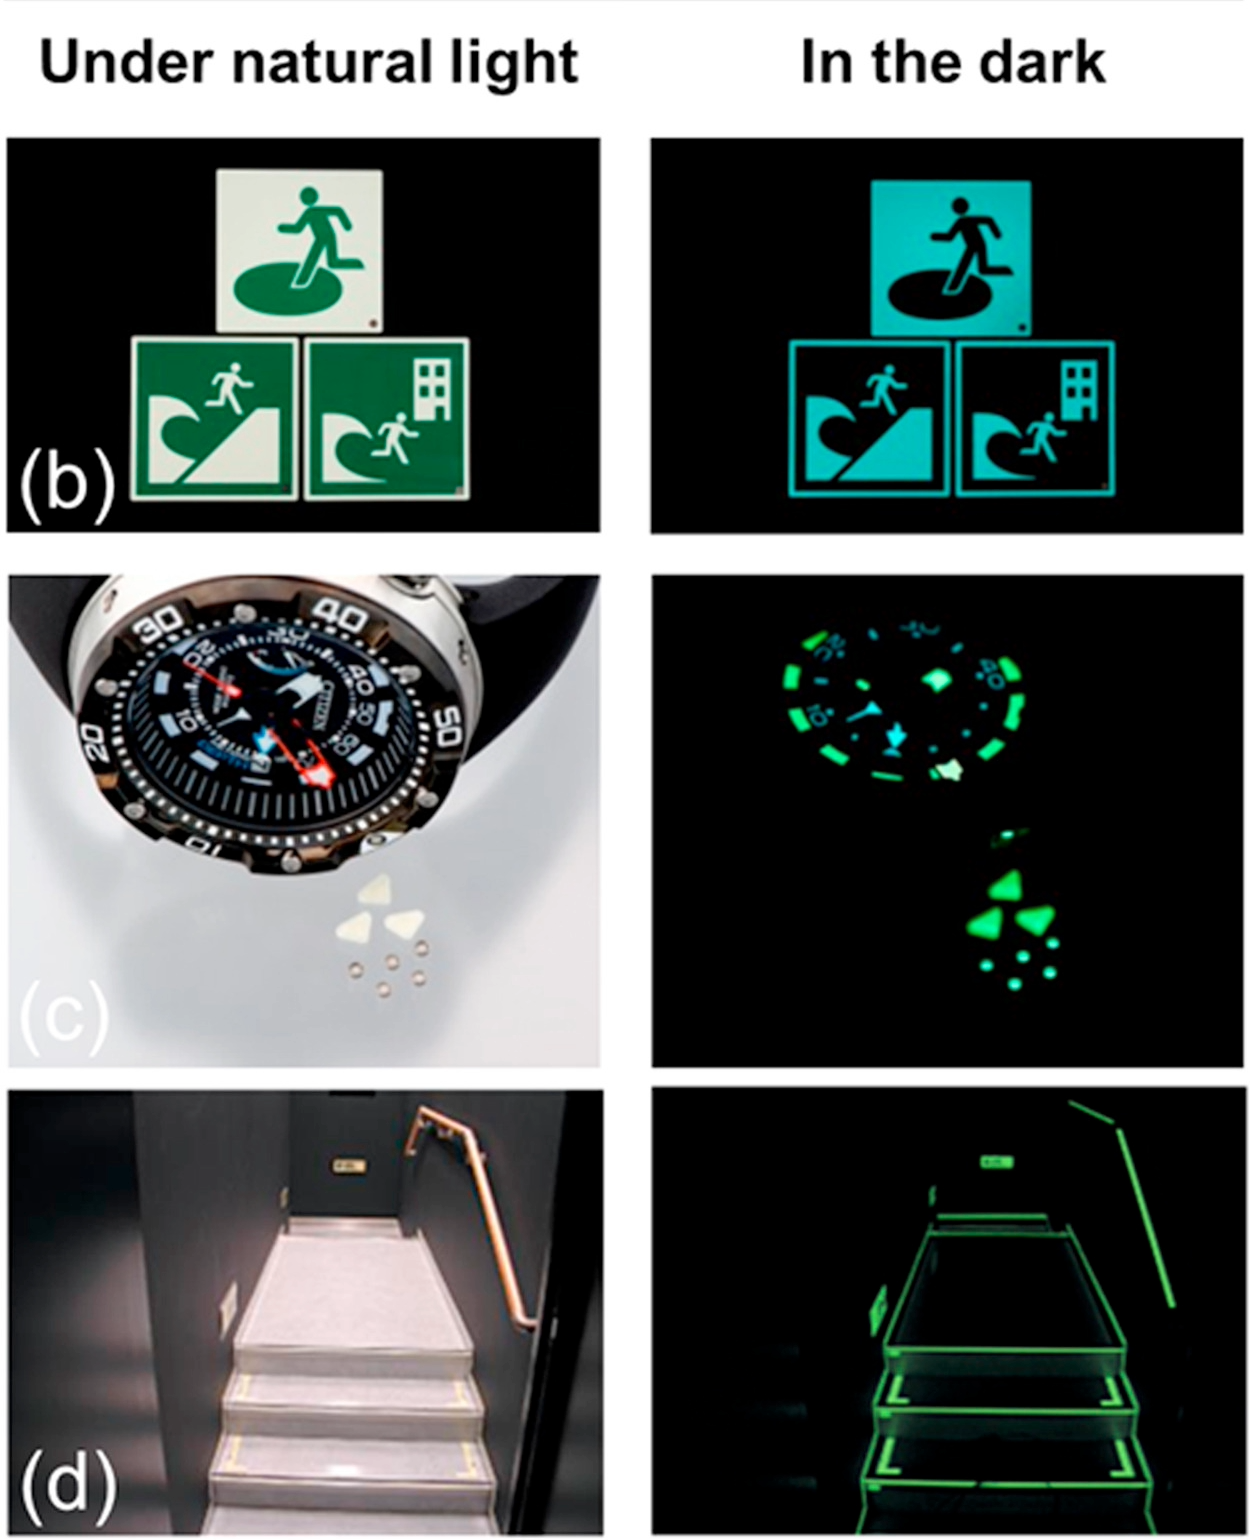
\includegraphics[height=9cm]{Luminova.png}
		\caption{Anwendung des persistenten Leuchtstoffs LumaNova\textsuperscript{\textregistered} in b{)} Rettungszeichen, c{) analogen Uhren, d{)} Farben zur Wegbeleuchtung.} \cite{xu_persistent_2019}}
	\end{figure}
	\chapter{Theoretischer Hintergrund} %max 2 Seiten
	
	\chapter{Resultate und Diskussion} %max 3 Seiten
	
	\chapter{Zusammenfassung} %max 1 Seite
	
	\listoffigures
	\addcontentsline{toc}{chapter}{Abbildungsverzeichnis}
	\printbibliography
	\end{document}
